% Titre : fonctions
% Filiere : BCPST
% Difficulte : 
% Type : TD 
% Categories :fonctions
% Subcategories : 
% Keywords : fonctions




\begin{exercice}  \;
\textbf{(Fonctions trigonom\'etriques)}
\noindent Soit $f$ une fonction d\'efinie par $f(x)=\ln{\left|  \cos{(x)}\sin{(x)} \right|}$.
\begin{enumerate}
\item D\'eterminer le domaine de d\'efinition $\mathcal{D}_f$ de $f$.
\item Montrer que $f$ est $\pi$ p\'eriodique, paire et que: $\forall x\in\mathcal{D}_f,\ f\left( \ddp\frac{\pi}{2}-x\right)=f(x)$. A quel intervalle peut-on r\'eduire l'\'etude de la fonction $f$ ?
\item Montrer soigneusement que $f$ est d\'erivable sur $\left \rbrack 0,\ddp\frac{\pi}{4}\right\rbrack$ et calculer sa d\'eriv\'ee. Dresser le tableau de variation de $f$ sur cet intervalle.
\item Tracer la courbe de $f$ en justifiant sa construction.
%\item Montrer que $f$ r\'ealise une bijection de $\left \rbrack 0,\ddp\frac{\pi}{4}\right\rbrack$ sur un intervalle \`{a} d\'eterminer. 
\end{enumerate}
\end{exercice}


\%\%\%\%\%\%\%\%\%\%\%\%\%\%\%\%\%\%\%\%
\%\%\%\%\%\%\%\%\%\%\%\%\%\%\%\%\%\%\%\%
\%\%\%\%\%\%\%\%\%\%\%\%\%\%\%\%\%\%\%\%



\begin{correction}  \;
\begin{enumerate}
\item La fonction $f$ est bien d\'efinie si et seulement si $\cos{x}\sin{x}\not= 0$. Or on a: $\cos{x}\sin{x}=0\Leftrightarrow \exists k\in\Z,\ x=\ddp\frac{\pi}{2}+k\pi\ \hbox{ou}\ \exists k\in\Z,\ x=k\pi$. Ainsi $\mathcal{D}_f=\R\setminus\left\lbrace \ddp\frac{\pi}{2}+k\pi,\ k\pi,\ k\in\Z\right\rbrace$.
\item R\'eduction d'intervalle:
\begin{itemize}
\item[$\bullet$] Montrons que $f$ est $\pi$ p\'eriodique : pour tout $x\in\mathcal{D}_f$, on a bien $x+\pi\in\mathcal{D}_f$ et $f(x+\pi)=\ln{ |  \cos{(x+\pi)} \sin{(x+\pi)} | }=\ln{| -\cos{x}\times (-\sin{x})| }=\ln{ | \cos{x}\sin{x} | }=f(x)$.
Ainsi la fonction $f$ est $\pi$ p\'eriodique et on peut restreindre l'intervalle d'\'etude \`{a} $\left\rbrack -\ddp\frac{\pi}{2},\ddp\frac{\pi}{2}\right\lbrack\setminus\lbrace 0\rbrace$.
\item[$\bullet$] Montrons que $f$ est paire: $\mathcal{D}_f$ est centr\'e en 0, et $\forall x\in\mathcal{D}_f$, on a: $f(-x)=\ln{ |  \cos{(-x)}\sin{(-x)} | }=\ln{  |  \cos{x}\times (-\sin{x})  | }=\ln{|  \cos{x} \sin{x}|}=f(x)$ en utilisant le fait que la fonction cosinus est paire, la fonction sinus impaire et le fait que $|-1|=1$.
Ainsi la fonction $f$ est paire et on peut restreindre l'\'etude \`{a} $\rbrack 0,\ddp\frac{\pi}{2}\lbrack$. 
\item[$\bullet$] Soit $x\in\mathcal{D}_f$, on a: $f\left(  \ddp\frac{\pi}{2}-x \right)=
 \ln{  |  \cos{ \left(  \ddp\frac{\pi}{2}-x \right)}  \sin{ \left(  \ddp\frac{\pi}{2}-x \right)  }  | } = \ln{ |  \sin{x}\cos{x}   |  }=f(x)  $ en utilisant le formulaire de trigonom\'etrie. \\
\noindent On peut faire un dessin pour s'en rendre compte mais une telle \'egalit\'e signifie que la droite d'\'equation 
$x=\ddp\frac{\pi}{4}$ est axe de sym\'etrie pour la courbe. Ainsi on peut \'etudier la fonction sur $\left\rbrack 0,\ddp\frac{\pi}{4}\right\rbrack$ puis faire la sym\'etrie d'axe $x=\ddp\frac{\pi}{4}$ pour obtenir la courbe sur $\rbrack 0,\ddp\frac{\pi}{2}\lbrack$.  
\end{itemize}
\item La fonction $x\mapsto \cos{x}\sin{x}$ est d\'erivable sur $\left\rbrack 0,\ddp\frac{\pi}{4}\right\rbrack$ comme produit de fonctions d\'erivables. De plus, sur cet ensemble, cette fonction ne s'annule pas. Comme la fonction valeur absolue est d\'erivable sur $\R^{\star}$, on obtient que $x\mapsto | \cos{x}\sin{x}|$ est d\'erivable sur $\left\rbrack 0,\ddp\frac{\pi}{4}\right\rbrack$ par composition. Comme sur cet intervalle, la fonction est \`{a} valeurs strictement positives et que la fonction logarithme n\'ep\'erien est d\'erivable sur $\R^{+\star}$, $f$ est bien d\'erivable sur $\left\rbrack 0,\ddp\frac{\pi}{4}\right\rbrack$ par composition.\\
\noindent De plus, en \'etudiant des cas, on sait que $(\ln{|u|})^{\prime}=\ddp\frac{u^{\prime}}{u}$ si $u$ d\'erivable. Ainsi ici on obtient que: $f^{\prime}(x)=\ddp\frac{  \cos^2{x} - \sin^2{x}  }{\cos{x} \sin{x}}=\ddp\frac{\cos{(2x)}}{\cos{x} \sin{x}} $.\\
\noindent Sur $\left\rbrack 0,\ddp\frac{\pi}{4}\right\rbrack$, on a: $\cos{x}> 0$, $\sin{x}>0$ et $\cos{(2x)}\geq 0$ car $2x\in \left\rbrack 0,\ddp\frac{\pi}{2}\right\rbrack$. Ainsi on a: $f^{\prime}(x)\geq 0$ sur $\left\rbrack 0,\ddp\frac{\pi}{4}\right\rbrack$.
\begin{center}
 \begin{tikzpicture}
 \tkzTabInit{ $x$          /1,%
       $f$       /1}%
     { $0$,$\ddp\frac{\pi}{4}$}%
  \tkzTabVar{
       -/$-\infty$            /,
        +/ $-\ln{2}$          /
                      }                
\end{tikzpicture}
\end{center}
En effet: $\lim\limits_{x\to 0^+} f(x)=-\infty$ par propri\'et\'es sur les produit et compos\'ees de limites. 
%\item Graphe de $f$ :
%\begin{center}
%\includegraphics[width=0.4\linewidth]{./ex14.eps} 
%\end{center}
%\item (\`A faire plus tard) On a
%\begin{itemize}
%\item[$\bullet$] La fonction $f$ est continue sur $\left\rbrack 0,\ddp\frac{\pi}{4}\right\rbrack$ comme produit et compos\'ee de fonctions continues.
%\item[$\bullet$] La fonction $f$ est strictement croissante sur $\left\rbrack 0,\ddp\frac{\pi}{4}\right\rbrack$.
%\item[$\bullet$] $\lim\limits_{x\to 0^+} f(x)=-\infty$ et $f\left(\ddp\frac{\pi}{4}\right)=-\ln{2}$.
%\end{itemize}
%Ainsi d'apr\`{e}s le th\'eor\`{e}me de la bijection, la fonction $f$ est bijective de $\left\rbrack 0,\ddp\frac{\pi}{4}\right\rbrack$ sur $\rbrack -\infty,-\ln{2}\rbrack$.
\end{enumerate}
\end{correction}

%------------------------------------------------
%------------------------------------------------
